\documentclass[table]{beamer}
\usetheme{Madrid}
\useinnertheme{rectangles}
\useoutertheme{infolines}
\usepackage{amsmath, amssymb, amsthm}

\usepackage [english]{babel}
\usepackage [autostyle, english = american]{csquotes}
\MakeOuterQuote{"}

\usepackage{graphicx}




\title{Landmark Mortality with NN}
\author{Bryan Cai}
\institute
{MIT}

\AtBeginSubsection[]
{
  \begin{frame}
    \frametitle{Table of Contents}
    \tableofcontents[currentsection, currentsubsection]
  \end{frame}
}

\begin{document}
\frame{\titlepage}

\section{Methods}

\subsection{Previous Work}

\begin{frame}
	\frametitle{Overview}
	\begin{itemize}
		\item Goal was to predict mortality based on data taken from the ICU
		\begin{itemize}
			\item Mortality was measured 30 days from the ICU entry date
		\end{itemize}
		\item Grouped related variables together
		\begin{itemize}
			\item Cardio, Chemistries, Hematology, Ventilation, UrineIO, and Miscellaneous groupings
		\end{itemize}
		\item Create mini models and calculate a separate mortality score for each patient using the groups of variables
		\item Consolidate the models into a super model
	\end{itemize}
\end{frame}

\begin{frame}
	\frametitle{Overview}
	\begin{center}
		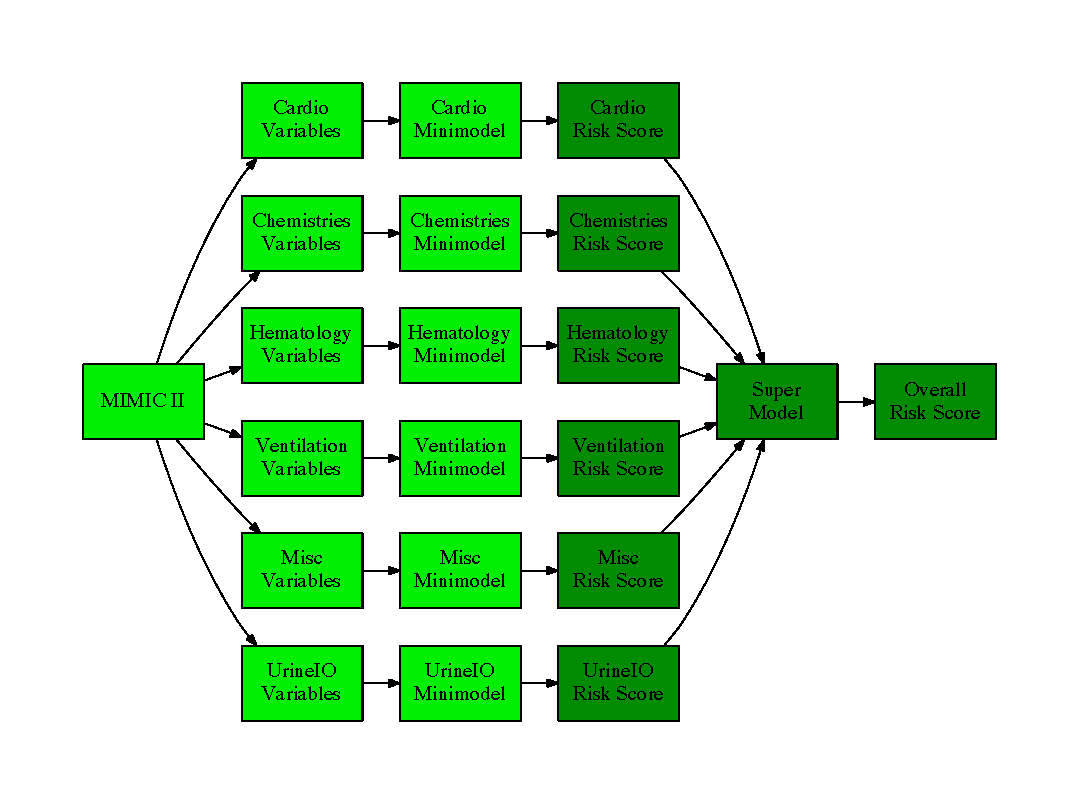
\includegraphics[height=8cm]{Images/Graphs/Overview.pdf}
	\end{center}
\end{frame}


\begin{frame}
	\frametitle{Landmarking}
	\begin{itemize}
		\item This procedure was performed for each distinct landmark time
		\begin{itemize}
			\item 8 hours, 1 day, and 2 day from ICU entry time
		\end{itemize}
		\item The model for landmark time $T$ aims to predict mortality for patients who have survived until time $T$ based on data up to time $T$
		\item Data retrieval and manipulation was done using Python
		\item Analysis was done using R
	\end{itemize}
\end{frame}

\begin{frame}
	\frametitle{Landmarking}
	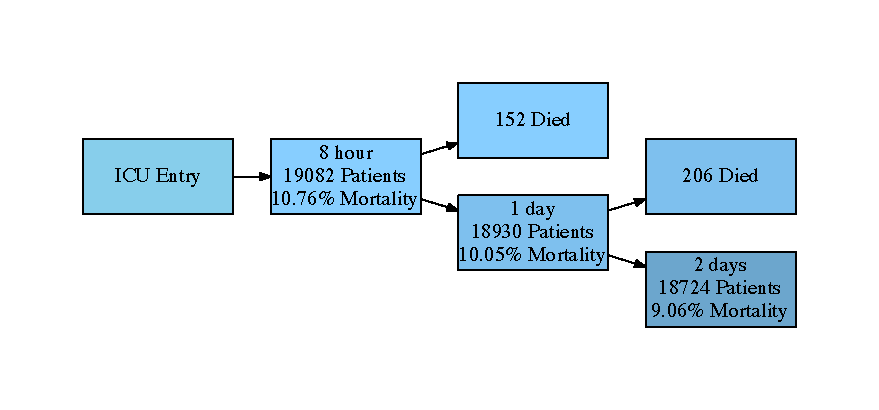
\includegraphics[height=6cm]{Images/Graphs/Landmark.pdf}
\end{frame}


\begin{frame}
	\frametitle{Data Filtering}
	\begin{itemize}
		\item For each landmark time $T$, we used the data where:
		\begin{itemize}
			\item The patient was still alive at time $T$, and
			\item The data was recorded before time $T$
		\end{itemize}
		\item Deleted variables where less than 5\% of patients had measurements taken
	\end{itemize}
\end{frame}

\begin{frame}
	\frametitle{Data Processing}
	\begin{itemize}
		\item For each variable $v$ and each patient, a set of summary variables were created:
		\begin{itemize}
			\item Calculated maximum, minimum, mean, median, median absolute deviation, number of measurements, and an indicator variable for whether any measurements took place
		\end{itemize}
		\item Imputed missing data using mean
	\end{itemize}
\end{frame}


\subsection{Current Work}

\begin{frame}
	\frametitle{Neural Network Structure}
	\begin{itemize}
		\item Tried several different network architectures
		\begin{itemize}
			\item Input $\to 500 \to 100 \to$ output
			\item Input $\to 1000 \to 500 \to$ output
			\item Input $\to 500 \to 700 \to 100 \to$ output
			\item Input $\to 100 \to$ output
		\end{itemize}
		\item Used ReLU as our activation function for the hidden layers
		\item Used the sigmoid function for the output layer
	\end{itemize}
\end{frame}

\begin{frame}
	\frametitle{Training and Loss Function}
	\begin{itemize}
		\item Applied dropout before the output layer to address overfitting
		\item Used binary cross entropy as our loss function
		\item The model is implemented in Torch
		\item Used Lutorpy to embed Torch code into Python for easy data manipulation
	\end{itemize}
\end{frame}

\section{Results}

%%%%%%%%%%%%%%%%%%%%%%%%%%%%%%%%%%%%%%%%%%%%%%%%%%%%%%%%%%%
%%%%%%%%%%%%%%%%%%%%%%%%%%%%%%%%%%%%%%%%%%%%%%%%%%%%%%%%%%%

\subsection{8 hours}

\begin{frame}
	\frametitle{Baseline}
	\begin{center}
		\begin{tabular}{c | c c}
			40,000 & LASSO & SVM \\ \hline
			AUC & 83.4\% & 80.7\% \\
		\end{tabular}
	\end{center}
\end{frame}

\begin{frame}
\frametitle{Overall}
\begin{columns}[c]
	\begin{column}{8cm}
		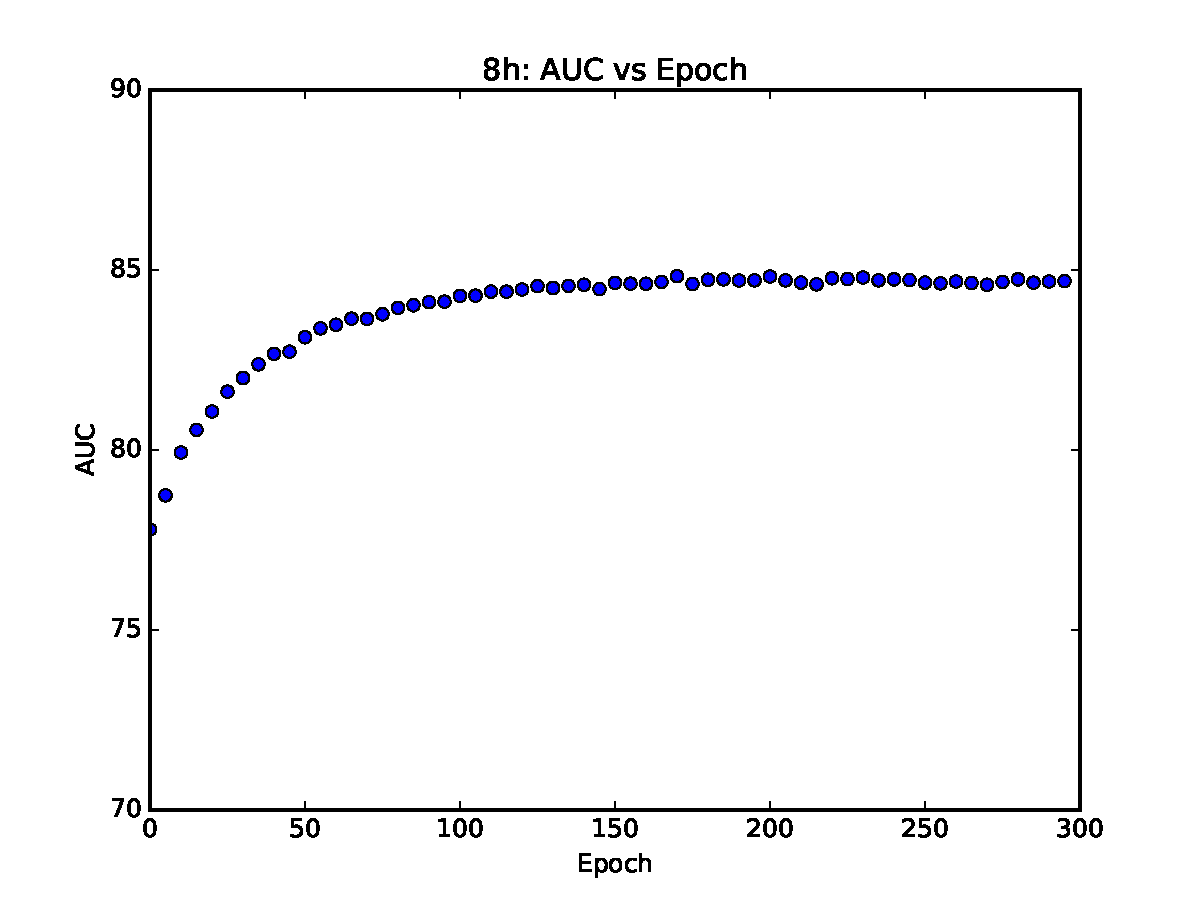
\includegraphics[width=8.5cm]{Images/NNplots/8h.pdf}
	\end{column}
\begin{column}{4cm}
Overall AUC: 84.5\%
\end{column}

\end{columns}
\end{frame}

\begin{frame}
	\frametitle{Two Layered}
	\begin{center}
		\begin{tabular}{c | c c c}
			40,000 & NN & LASSO & SVM \\ \hline
			NN & 82.2\% & \textbf{83.1\%} & 79.3\% \\
			LASSO & 77.4\% & 76.7\% & 72.7\% \\
			SVM & 78.2\% & 79.2\% & 75.2\%
		\end{tabular}
	
		\framebox{Highest Achieved: 85.0\% (NN-NN)}
	\end{center}
\end{frame}

%%%%%%%%%%%%%%%%%%%%%%%%%%%%%%%%%%%%%%%%%%%%%%%%%%%%%%%%%%%
%%%%%%%%%%%%%%%%%%%%%%%%%%%%%%%%%%%%%%%%%%%%%%%%%%%%%%%%%%%

\subsection{1 day}

\begin{frame}
	\frametitle{Baseline}
	\begin{center}
		\begin{tabular}{c | c c}
			40,000 & LASSO & SVM \\ \hline
			AUC & 85.0\% & 81.3\% \\
		\end{tabular}
	\end{center}
\end{frame}

\begin{frame}
	\frametitle{Overall}
	\begin{columns}[c]
		\begin{column}{8cm}
			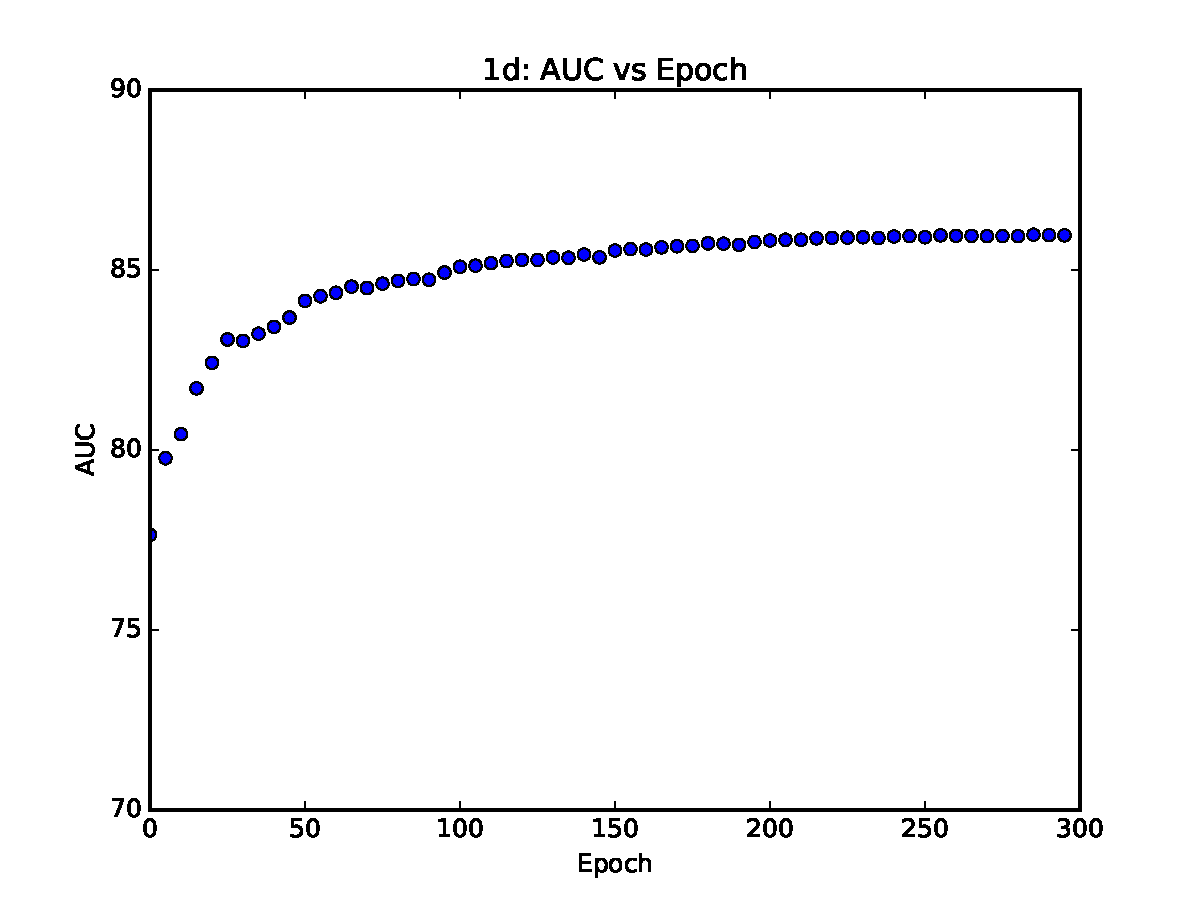
\includegraphics[width=8.5cm]{Images/NNplots/1d.pdf}
		\end{column}
		\begin{column}{4cm}
			Overall AUC: 85.9\%
		\end{column}
		
	\end{columns}
\end{frame}

\begin{frame}
	\frametitle{Two Layered}
	\begin{center}
		\begin{tabular}{c | c c c}
			40,000 & NN & LASSO & SVM \\ \hline
			NN & 83.9\% & 86.3\% & 79.7\% \\
			LASSO & 84.8\% & 83.8\% & 78.7\% \\
			SVM & 83.9\% & \textbf{86.4\%} & 77.2\%
		\end{tabular}
	
		\framebox{Highest Achieved: 88.7\% (LASSO-NN)}
	\end{center}
\end{frame}

%%%%%%%%%%%%%%%%%%%%%%%%%%%%%%%%%%%%%%%%%%%%%%%%%%%%%%%%%%%
%%%%%%%%%%%%%%%%%%%%%%%%%%%%%%%%%%%%%%%%%%%%%%%%%%%%%%%%%%%

\subsection{2 days}

\begin{frame}
	\frametitle{Baseline}
	\begin{center}
		\begin{tabular}{c | c c}
			40,000 & LASSO & SVM \\ \hline
			AUC & 85.1\% & 83.3\% \\
		\end{tabular}
	\end{center}
\end{frame}

\begin{frame}
	\frametitle{Overall}
	\begin{columns}[c]
		\begin{column}{8cm}
			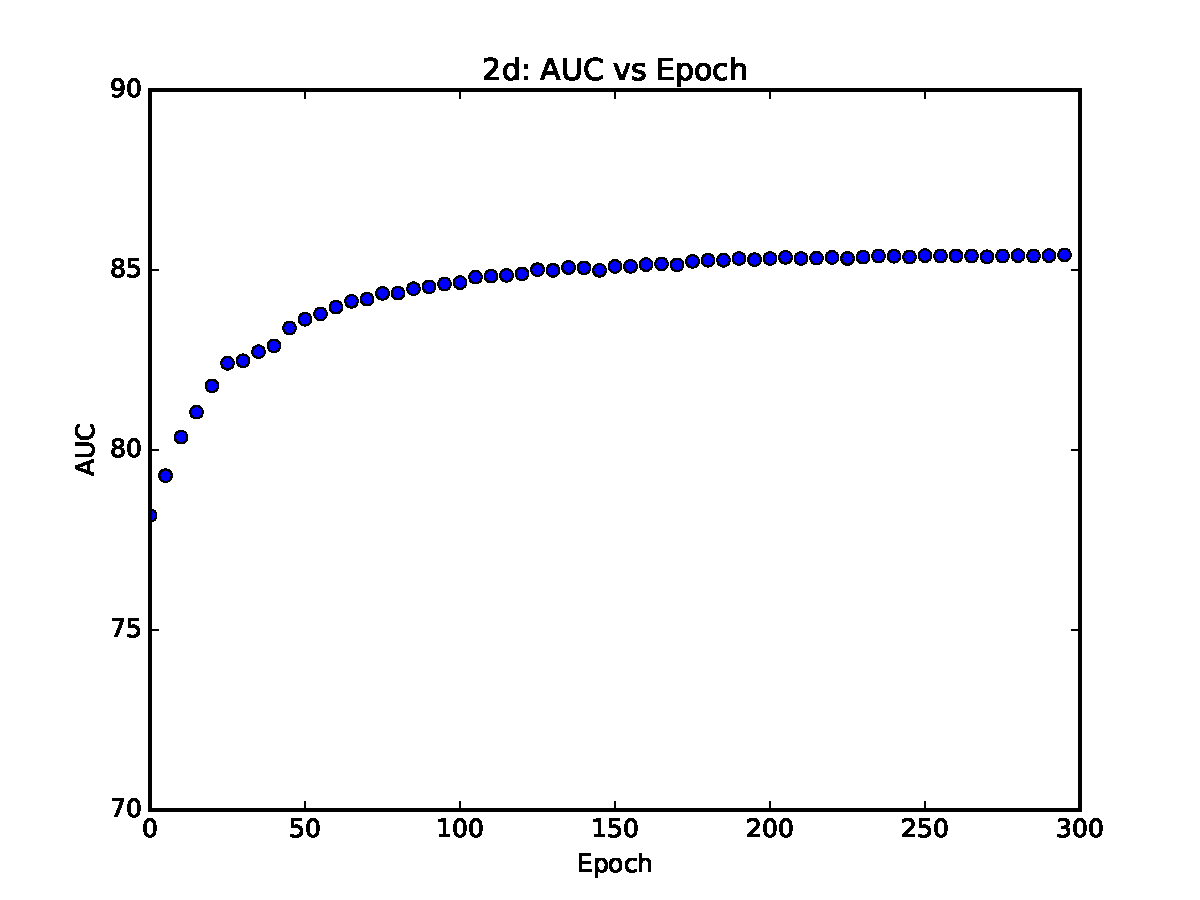
\includegraphics[width=8.5cm]{Images/NNplots/2d.pdf}
		\end{column}
		\begin{column}{4cm}
			Overall AUC: 85.4\%
		\end{column}
		
	\end{columns}
\end{frame}

\begin{frame}
	\frametitle{Two Layered}
	\begin{center}
		\begin{tabular}{c | c c c}
			40,000 & NN & LASSO & SVM \\ \hline
			NN & \textbf{85.6\%} & 82.5\% & 81.6\% \\
			LASSO & 83.2\% & 83.9\% & 79.2\% \\
			SVM & 81.2\% & 82.1\% & 76.5\%
		\end{tabular}
	
		\framebox{Highest Achieved: 87.7\% (NN-NN)}
	\end{center}
\end{frame}


\end{document}